\chapter{Metrics, Expansion, and a First Cosmology}

At the end of the preceding lecture we had reached a Lorentz-invariant wave
equation and were preparing to write Maxwell's equations in spacetime form.
An audience question now supplies a useful warning before we turn to
gravitation: how much of a physical theory can symmetry determine by itself?
The answer is emphatic: a great deal, but not everything. Lorentz invariance
is a powerful filter on possible laws. It is not a substitute for the
remaining physical assumptions or for experiment.

\section{What symmetry does not determine}

\begin{classroomqa}
\audiencequestion{Once the electric and magnetic fields are known to
transform together under Lorentz transformations, do Maxwell's equations
follow from relativity alone?}
\lecturerresponse{No. Relativity constrains the form of the equations, but
the construction also uses their linearity, the low order of their
derivatives, the way the fields transform, and experimental information.
Without those additional ingredients many Lorentz-covariant field equations
would still be possible.}
\end{classroomqa}

The most important of those extra assumptions for the opening discussion is
linearity. If \(A(x,t)\) is a solution of a linear field equation, then
\(\lambda A(x,t)\) is also a solution for every constant \(\lambda\). If
\(A\) and \(B\) are solutions, then so is
\begin{equation}
  C(x,t)=A(x,t)+B(x,t).
  \label{eq:superposition}
\end{equation}
This is the superposition principle. Two source-free electromagnetic waves
may cross one another and emerge unchanged. They do not collide directly in
the way material objects do. They can interact indirectly through charged
matter, because each wave moves the charges and the moving charges radiate,
but the vacuum field equations themselves are linear.

\begin{figure}[H]
\centering

\includegraphics[width=0.64\textwidth]{lecture_08_figure_01.png}
\caption{Two wave profiles on the board during the discussion of
superposition. Their sum is again an allowed source-free wave.}
\lectureframe{00:05:30}
\end{figure}

The harmonic oscillator makes the algebra transparent. Suppose
\begin{equation}
  m\ddot x=-kx.
  \label{eq:linear-oscillator}
\end{equation}
If \(x_1\) and \(x_2\) solve \eqref{eq:linear-oscillator}, then
\begin{equation}
  m(\ddot x_1+\ddot x_2)
  =-k(x_1+x_2),
\end{equation}
so \(x_1+x_2\) is a solution. Add a nonlinear term, however,
\begin{equation}
  m\ddot x=-kx+p x^2,
  \label{eq:nonlinear-oscillator}
\end{equation}
and the sum no longer works:
\begin{equation}
  (x_1+x_2)^2=x_1^2+x_2^2+2x_1x_2.
\end{equation}
The cross term \(2x_1x_2\) has no counterpart in the two separate
equations. The two motions now influence one another.

\begin{figure}[H]
\centering

\includegraphics[width=0.73\textwidth]{lecture_08_figure_02.png}
\caption{Separate oscillator equations compared with the equation for their
sum. The quadratic term exposes the extra cross term that breaks
superposition.}
\lectureframe{00:10:10}
\end{figure}

This example fixes the methodological point that will remain in force
throughout the cosmology discussion. Symmetry tells us which quantities may
be combined and which equations are allowed. Dynamics and observation tell
us which allowed equation nature uses.

\section{The interval as geometry}

We now leave electromagnetism and take a short route into general relativity
and cosmology. The starting object is the interval between neighboring
events. Label an event by four coordinates \(x^\mu\) and a nearby event by
\(x^\mu+dx^\mu\). In inertial Cartesian coordinates, with \(c=1\) and the
\((+,-,-,-)\) convention,
\begin{equation}
  d\tau^2
  =dt^2-dx^2-dy^2-dz^2
  =dx^\mu dx_\mu
  =\eta_{\mu\nu}\,dx^\mu dx^\nu.
  \label{eq:minkowski-interval}
\end{equation}
The quantity \(d\tau^2\), not any one coordinate difference, is invariant.
Lorentz transformations change \(dt,dx,dy,dz\) while preserving this
quadratic combination. Special relativity may therefore be read as the
geometry of Minkowski spacetime.

\begin{figure}[H]
\centering

\includegraphics[width=0.72\textwidth]{lecture_08_figure_03.png}
\caption{The Minkowski interval written successively in component,
contracted-index, and metric-tensor notation.}
\lectureframe{00:14:50}
\end{figure}

The simplicity of \eqref{eq:minkowski-interval} depends on the coordinates.
Even a flat plane can acquire unfamiliar coefficients if we label it
unwisely. Let \(x\) be measured in centimeters while \(y\) is measured in
meters. For a physical displacement,
\begin{equation}
  ds^2=dx^2+\left(\frac{dy}{100}\right)^2
      =dx^2+10^{-4}dy^2.
  \label{eq:mixed-units}
\end{equation}
The factor \(10^{-4}\) says nothing about curvature. It merely translates
between units.

\begin{figure}[H]
\centering

\includegraphics[width=0.59\textwidth]{lecture_08_figure_04.png}
\caption{A flat plane described with centimeters on one axis and meters on
the other. The unequal metric coefficients encode units, not curvature.}
\lectureframe{00:20:10}
\end{figure}

Oblique coordinates add a mixed term. In two dimensions the most general
local quadratic form can be written
\begin{equation}
  ds^2
  =a_{11}\,dx^2+a_{12}\,dx\,dy
   +a_{21}\,dy\,dx+a_{22}\,dy^2,
  \qquad a_{12}=a_{21}.
  \label{eq:quadratic-form}
\end{equation}
Because ordinary differentials commute, \(dx\,dy=dy\,dx\), only the
symmetric part of the coefficient array contributes. We collect the
coefficients into the matrix
\begin{equation}
  g=
  \begin{pmatrix}
    a_{11} & a_{12}\\
    a_{21} & a_{22}
  \end{pmatrix}.
  \label{eq:metric-matrix}
\end{equation}
This matrix is the \emph{metric}. It is the local rule that converts
coordinate differences into physical intervals.

\begin{figure}[H]
\centering

\includegraphics[width=0.71\textwidth]{lecture_08_figure_05.png}
\caption{The quadratic differential form and its symmetric \(2\times2\)
coefficient matrix at the moment the matrix is identified as the metric.}
\lectureframe{00:24:07}
\end{figure}

Uniform rectangular or oblique grids give constant coefficients. If the
coordinate lines curve, bunch together, or spread apart, those coefficients
become functions of position even when the underlying surface remains flat.
The general spacetime notation is
\begin{equation}
  ds^2=g_{\mu\nu}(x)\,dx^\mu dx^\nu.
  \label{eq:general-metric}
\end{equation}

\begin{figure}[H]
\centering

\includegraphics[width=0.66\textwidth]{lecture_08_figure_06.png}
\caption{The general position-dependent metric after the coordinate grid is
allowed to vary from point to point.}
\lectureframe{00:28:10}
\end{figure}

Knowing \(g_{\mu\nu}\) in a specified coordinate system determines local
distances, times, and angles and thereby determines the geometry. The
converse is not unique: one geometry has infinitely many coordinate
descriptions, hence infinitely many arrays of coefficient functions related
by coordinate transformations.

\section{Coordinate complexity and intrinsic curvature}

We must now distinguish a complicated metric from a curved space. Roll a
sheet of paper into a cylinder without stretching it. Its appearance in the
room changes, but all distances measured within the sheet remain the same.
A creature confined to the paper cannot detect the bending by any intrinsic
measurement. That is extrinsic bending, not the curvature meant here.

A hemisphere is different. It cannot be pressed flat without stretching,
tearing, or compressing it. A flat map of Earth must distort either distance,
area, angle, or some combination of them. This obstruction is intrinsic and
can be detected without looking into a surrounding dimension.

Polar coordinates give the indispensable flat counterexample. On a plane,
an infinitesimal radial displacement has length \(dr\), while an angular
displacement \(d\theta\) at radius \(r\) has length \(r\,d\theta\). Thus
\begin{equation}
  ds^2=dr^2+r^2d\theta^2,
  \qquad
  g_{\text{polar}}=
  \begin{pmatrix}
    1&0\\
    0&r^2
  \end{pmatrix}.
  \label{eq:polar-metric}
\end{equation}
The coefficient \(r^2\) varies across the plane, yet the plane is flat. The
change of variables
\begin{equation}
  x=r\cos\theta,\qquad y=r\sin\theta
\end{equation}
returns the constant metric \(ds^2=dx^2+dy^2\).

\begin{figure}[H]
\centering

\includegraphics[width=0.70\textwidth]{lecture_08_figure_07.png}
\caption{The polar metric and its return to the Cartesian metric. The
position-dependent matrix on the left still describes a flat plane.}
\lectureframe{00:39:20}
\end{figure}

\begin{classroomqa}
\audiencequestion{Should the angular distance in polar coordinates contain
a sine?}
\lecturerresponse{Not on the plane. There the arc length is
\(r\,d\theta\). A sine appears on the sphere, where a circle of latitude has
radius \(R\sin\theta\).}
\end{classroomqa}

Take a sphere of radius \(R\). Let \(\theta\) be the polar angle measured
from the north pole and \(\phi\) the azimuthal angle. A meridional step has
length \(R\,d\theta\). At polar angle \(\theta\), the circle of latitude has
radius \(R\sin\theta\), so an azimuthal step has length
\(R\sin\theta\,d\phi\). Local Pythagoras gives
\begin{equation}
  ds^2
  =R^2\left(d\theta^2+\sin^2\theta\,d\phi^2\right),
  \qquad
  g_{\text{sphere}}=
  \begin{pmatrix}
    R^2&0\\
    0&R^2\sin^2\theta
  \end{pmatrix}.
  \label{eq:sphere-metric}
\end{equation}

\begin{figure}[H]
\centering

\includegraphics[width=0.72\textwidth]{lecture_08_figure_08.png}
\caption{The sphere, its angular line element, and the corresponding metric
matrix. The \(\sin^2\theta\) factor records the shrinking circles of
latitude.}
\lectureframe{00:45:15}
\end{figure}

\begin{figure}[H]
\centering
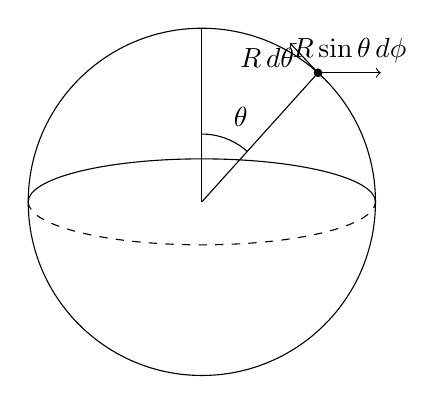
\begin{tikzpicture}[scale=1.05]
  \draw (0,0) circle (2.1);
  \draw[dashed] (-2.1,0) arc (180:360:2.1 and 0.52);
  \draw (2.1,0) arc (0:180:2.1 and 0.52);
  \coordinate (P) at (48:2.1);
  \fill (P) circle (1.5pt);
  \draw (0,0) -- (0,2.1);
  \draw (0,0) -- (P);
  \draw (0,0.82) arc (90:48:0.82);
  \node at (0.47,1.03) {\(\theta\)};
  \draw[->] (P) -- ++(-0.34,0.36)
    node[midway,left] {\(R\,d\theta\)};
  \draw[->] (P) -- ++(0.76,0)
    node[midway,above] {\(R\sin\theta\,d\phi\)};
\end{tikzpicture}
\caption{Clean reconstruction of the local differential legs used to obtain
\eqref{eq:sphere-metric}.}
\end{figure}

No global change of coordinates turns \eqref{eq:sphere-metric} into a
constant Euclidean matrix. A two-dimensional observer can discover this
intrinsically: a sufficiently large triangle made from geodesics has an
angle sum greater than \(180^\circ\). We have therefore reached the useful
criterion. Variable coefficients do not by themselves imply curvature.
Curvature is the obstruction to finding coordinates that make the metric
constant throughout the region under consideration.

\section{From curved spacetime to cosmology}

General relativity permits spacetime itself to possess this intrinsic
curvature. A position-dependent \(g_{\mu\nu}\) may still be an artifact of
coordinates, as in polar coordinates, but in a genuinely curved spacetime no
coordinate transformation removes the variation globally.

\begin{figure}[H]
\centering

\includegraphics[width=0.70\textwidth]{lecture_08_figure_09.png}
\caption{The transition from special coordinate examples to the general
spacetime line element \(ds^2=g_{\mu\nu}(x)dx^\mu dx^\nu\).}
\lectureframe{00:48:40}
\end{figure}

We will not attempt the full machinery of Einstein's equations. Instead we
restrict attention to geometries appropriate to cosmology: space is taken
to be homogeneous on sufficiently large scales, while the geometry may
change with time. Homogeneous means that no location is distinguished from
another. It does not mean flat: every point on a sphere is equivalent, yet
the sphere is curved. It does not mean featureless on every scale either.

\begin{classroomqa}
\audiencequestion{How can the universe be homogeneous when galaxies form
clusters, sheets, and filaments?}
\lecturerresponse{The claim concerns coarse-grained scales. Stars, galaxies,
and clusters are strongly inhomogeneous. When regions hundreds of millions
of light-years across are compared, those structures average toward a
uniform distribution. The cosmological principle is an empirical working
hypothesis, not a logical necessity; sufficiently large systematic
differences, including directional differences in the cosmic background,
could disprove it.}
\end{classroomqa}

The second large-scale assumption in this lecture is spatial flatness. At a
fixed cosmic time, sufficiently large triangles appear Euclidean: their
angles add to \(180^\circ\). This is a statement about the geometry of
three-dimensional space, not yet about the curvature of four-dimensional
spacetime.

\begin{classroomqa}
\audiencequestion{What does simultaneity mean for points separated by
cosmological distances, since their light reaches us at different times?}
\lecturerresponse{We cannot place rods between distant galaxies or inspect
them instantaneously. We receive signals later and reconstruct the geometry
of the emitting events within a spacetime model. The procedure is indirect,
but so are many geometric measurements in astronomy. Flatness means that
the reconstructed large triangles show no detectable angular excess or
deficit on the surveyed scale.}
\end{classroomqa}

\section{Comoving coordinates and the scale factor}

Imagine a Cartesian grid painted onto the large-scale flow of galaxies.
Each galaxy keeps its coordinate label as the grid expands. The label is not
a distance in meters; it is an address. A time-dependent conversion factor
turns coordinate separations into physical separations.

\begin{figure}[H]
\centering
\begin{tikzpicture}[>=Latex,scale=0.86]
  \foreach \x in {0,0.65,1.3,1.95,2.6} {
    \draw[gray!65] (\x,0) -- (\x,2.2);
  }
  \foreach \y in {0,0.55,1.1,1.65,2.2} {
    \draw[gray!65] (0,\y) -- (2.6,\y);
  }
  \fill[blue!65!black] (0.65,0.55) circle (2pt);
  \fill[red!70!black] (1.95,1.65) circle (2pt);
  \node[below] at (1.3,-0.2) {comoving labels at \(t_1\)};
  \draw[->,very thick] (3.0,1.1) -- (4.0,1.1)
    node[midway,above] {\(a(t)\) grows};
  \foreach \x in {4.4,5.5,6.6,7.7,8.8} {
    \draw[gray!65] (\x,0) -- (\x,2.2);
  }
  \foreach \y in {0,0.55,1.1,1.65,2.2} {
    \draw[gray!65] (4.4,\y) -- (8.8,\y);
  }
  \fill[blue!65!black] (5.5,0.55) circle (2pt);
  \fill[red!70!black] (7.7,1.65) circle (2pt);
  \node[below] at (6.6,-0.2) {same labels at \(t_2\)};
\end{tikzpicture}
\caption{The comoving addresses stay fixed while the physical spacing of
the coordinate grid grows.}
\end{figure}

Spatial homogeneity requires the same conversion factor everywhere at a
given time. Spatial flatness allows the spatial part of the metric to be
Cartesian. The resulting line element is
\begin{equation}
  d\tau^2
  =dt^2-a^2(t)\left(dx^2+dy^2+dz^2\right).
  \label{eq:flrw-flat}
\end{equation}
This is the spatially flat homogeneous cosmological metric in comoving
coordinates. We may choose \(x,y,z\) dimensionless and give \(a(t)\) units
of length. Another convention can put the dimensions into the coordinates
and make \(a\) dimensionless; only the product matters.

\begin{figure}[H]
\centering

\includegraphics[width=0.76\textwidth]{lecture_08_figure_10.png}
\caption{The spatially flat cosmological metric as completed on the board,
with the common factor \(a^2(t)\) multiplying all three spatial
directions.}
\lectureframe{01:03:15}
\end{figure}

If \(a\) were constant, we could absorb it by rescaling \(x,y,z\), and
\eqref{eq:flrw-flat} would be ordinary Minkowski spacetime in different
units. Its time dependence is the nontrivial ingredient.

\begin{classroomqa}
\audiencequestion{If the coordinate grid expands, why do meter sticks,
atoms, and galaxies not expand with it?}
\lecturerresponse{The metric describes the average cosmic flow, not a force
that compels every bound system to follow it. Electromagnetic forces hold a
meter stick and an atom together; self-gravity holds a galaxy together.
Those binding effects dominate the exceedingly weak background expansion
on small scales. Nearby galaxies can also depart from the Hubble flow:
Andromeda is pulled toward the Milky Way. Detailed studies of galactic
binding show that visible matter alone is insufficient, one of the
arguments for dark matter.}
\end{classroomqa}

\begin{classroomqa}
\audiencequestion{Why is the scale factor not itself a force that pushes
galaxies apart?}
\lecturerresponse{It has the dimensions of length in the present
convention, not force. Think of a cannonball launched upward. Once launched,
its outward motion is inertial; gravity changes that motion by reducing its
speed or pulling it back. Likewise, expansion is a state of motion. The
dynamical question is how gravity and other sources change \(\dot a\) and
\(\ddot a\), not what force is required to keep \(a\) moving.}
\end{classroomqa}

The old expectation was that attractive gravity should decelerate the
expansion. By the time of this lecture, astronomical evidence had shown that
the recent expansion is instead accelerating, which means that the complete
dynamics contains more than ordinary attractive matter. We postpone that
issue until the geometrical setup is secure.

\section{The Hubble law}

Take two comoving galaxies whose fixed coordinate separation is
\(\Delta x\). At a common cosmic time their physical distance is
\begin{equation}
  D(t)=a(t)\,\Delta x.
  \label{eq:physical-distance}
\end{equation}
Differentiate while holding the comoving labels fixed:
\begin{align}
  V(t)
    &=\dot D(t)
      =\dot a(t)\,\Delta x \nonumber\\
    &=\frac{\dot a(t)}{a(t)}D(t).
  \label{eq:hubble-derivation}
\end{align}
Define
\begin{equation}
  H(t)=\frac{\dot a(t)}{a(t)}.
  \label{eq:hubble-parameter}
\end{equation}
Then
\begin{equation}
  V(t)=H(t)D(t).
  \label{eq:hubble-law}
\end{equation}
At one cosmic time the same \(H(t)\) applies everywhere; otherwise space
would not be homogeneous. The recession speed is proportional to distance
because every interval in the comoving grid is stretched by the same
fractional rate.

\begin{figure}[H]
\centering

\includegraphics[width=0.73\textwidth]{lecture_08_figure_11.png}
\caption{Physical distance \(D=a\Delta x\) and its time derivative on the
way to \(V=(\dot a/a)D\).}
\lectureframe{01:16:45}
\end{figure}

\begin{classroomqa}
\audiencequestion{For a distant galaxy, should the Hubble parameter be
evaluated now or when the observed light was emitted?}
\lecturerresponse{At the epoch being described. Light from a distant galaxy
reports an earlier value of the expansion. A serious analysis must account
for the time dependence of \(H\); inserting today's value everywhere is
only a local approximation.}
\end{classroomqa}

\begin{classroomqa}
\audiencequestion{Where do the units reside in \(D=a\Delta x\)?}
\lecturerresponse{A convenient choice is to treat the comoving label
\(\Delta x\) as dimensionless and let \(a\) carry length. The opposite
bookkeeping is possible. Either way, \(H=\dot a/a\) has dimensions of
inverse time.}
\end{classroomqa}

\section{Light in the expanding coordinates}

Light follows a null path. Along such a path the proper-time interval
vanishes:
\begin{equation}
  d\tau^2=0.
\end{equation}

\begin{classroomqa}
\audiencequestion{Why is the interval zero for light?}
\lecturerresponse{That is the defining geometry of a light ray in
relativity. Every local freely falling observer measures light to move at
\(c=1\), so \(dt^2=d\ell^2\) locally and the spacetime interval vanishes.
It does not mean that no coordinate time passes for the observer receiving
the light.}
\end{classroomqa}

For a ray moving only in the \(x\)-direction,
\begin{equation}
  0=dt^2-a^2(t)\,dx^2.
\end{equation}
Choosing the ray that moves toward increasing \(x\),
\begin{equation}
  dt=a(t)\,dx,
  \qquad
  dx=\frac{dt}{a(t)},
  \qquad
  \frac{dx}{dt}=\frac{1}{a(t)}.
  \label{eq:null-ray}
\end{equation}

\begin{figure}[H]
\centering

\includegraphics[width=0.64\textwidth]{lecture_08_figure_12.png}
\caption{The null condition in the expanding metric and the resulting
comoving light-ray equation \(dx=dt/a(t)\).}
\lectureframe{01:23:45}
\end{figure}

The coordinate speed \(dx/dt\) decreases as the scale factor grows. This
does not mean that light locally slows down. One unit of comoving coordinate
distance represents an ever larger physical distance, so the numerical
coordinate speed changes while every local measurement still gives
\(c=1\).

\section{Why the time dependence matters}

The central geometrical question is now unavoidable: how does \(a(t)\)
vary? The analogy is a projectile whose position is known at one instant.
Its future trajectory requires an equation of motion. In cosmology,
gravitational dynamics will supply the equation for \(a(t)\).

\begin{classroomqa}
\audiencequestion{Why privilege the question whether \(a(t)\) changes over
the equally legitimate question whether, for example, the electron charge
changes with time?}
\lecturerresponse{There is no logical hierarchy. A measured change in the
electron charge would be enormously important. We focus on \(a(t)\) because
observation already tells us that cosmic separations change, whereas the
electron charge appears constant. Geometrically, a constant \(a\) could be
removed by a change of spatial units and would leave flat spacetime; a
time-dependent \(a\) cannot be removed that way.}
\end{classroomqa}

Before measuring distant recession, one needs this geometrical framework to
say what is being measured. At the crudest level, a source of known
luminosity appears dimmer with distance because its light spreads over a
larger area, while the displacement of known atomic spectral lines gives a
redshift and hence a recession indicator. Hubble combined distance
estimates with redshifts to uncover the proportionality
\eqref{eq:hubble-law}, although the early numerical value of the coefficient
was substantially wrong. Modern distance ladders and relativistic
light-propagation calculations are much more elaborate, but the conceptual
pair remains distance plus redshift.

\section{The Hubble time and the age estimate}

There is a simple estimate hidden in the Hubble law. Freeze a galaxy's
present recession speed and run the motion backward uniformly. The time
required to close its present distance would be
\begin{equation}
  t=\frac{D}{V}.
\end{equation}
Using \(V=HD\),
\begin{equation}
  t=\frac{D}{HD}=\frac{1}{H}.
  \label{eq:hubble-time}
\end{equation}
The distance cancels, so every pair of comoving galaxies gives the same
rough time. Susskind catches and corrects an easy verbal error here. The
assumption is not that \(H\) remains constant. It is that the particular
recession velocity is extrapolated backward as though it were constant.

\begin{figure}[H]
\centering

\includegraphics[width=0.66\textwidth]{lecture_08_figure_13.png}
\caption{The Hubble-time estimate \(H^{-1}=D/(HD)=D/V\), with distance
canceling from the backward extrapolation.}
\lectureframe{01:33:45}
\end{figure}

The inverse Hubble parameter is therefore a time scale, not automatically
the exact age of the universe. In a purely decelerating, matter-dominated
picture, reverse the present velocity and let gravity pull the galaxies
together. They meet sooner than they would at uniform velocity, so the
present \(H^{-1}\) overestimates the age. The lecture quotes a refined age of
about \(13.5\) billion years, close to the Hubble time but not identical to
it.

\begin{classroomqa}
\audiencequestion{If there is no Hubble expansion inside our galaxy, what
does it mean to run all galaxies backward until they collapse?}
\lecturerresponse{The homogeneous description eventually ceases to resolve
the real history of bound structures. Forward in time, small fluctuations
grow gravitationally into galaxies and clusters. A literal reversed movie
would require every microscopic motion to reverse and entropy to decrease;
simply reversing the average Hubble flow does not undo structure formation.
The backward extrapolation is a coarse cosmological estimate, not a film of
every star retracing its path.}
\end{classroomqa}

\begin{classroomqa}
\audiencequestion{Can an experiment distinguish an expanding intergalactic
distance from a shrinking ruler?}
\lecturerresponse{Only dimensionless ratios are observable. What is measured
is that the distance between galaxies divided by an atomic or laboratory
length standard increases. We conventionally hold the parameters of atomic
and molecular physics fixed and say that the universe expands. One could
choose the intergalactic separation as the standard and describe atoms,
protons, and meter sticks as shrinking. The physics of the ratio would be
unchanged.}
\end{classroomqa}

That convention is natural because rods are made from atoms and their size
is controlled by parameters that appear constant. A meter is ultimately a
large number of microscopic lengths. Holding those microscopic standards
fixed gives the familiar statement that \(a(t)\) grows.

\begin{classroomqa}
\audiencequestion{Is \eqref{eq:flrw-flat} the only metric compatible with
spatial homogeneity and flatness?}
\lecturerresponse{Only up to coordinate transformations. The precise claim
is that, under those assumptions and a suitable choice of cosmic time and
comoving spatial coordinates, the metric can be brought to this form.
Another coordinate system may make the same spacetime look quite
different.}
\end{classroomqa}

\begin{classroomqa}
\audiencequestion{When the backward separation reaches zero, the Hubble law
also gives zero velocity. Does that prevent the galaxies from meeting?}
\lecturerresponse{No. The \(H\) inferred today is not held fixed all the way
back. In ordinary expanding solutions \(H(t)\) was much larger at earlier
times. The estimate \(H_0^{-1}\) is made by extending today's velocity
uniformly only to obtain a scale; the real \(a(t)\), \(H(t)\), and velocities
must be found from dynamics.}
\end{classroomqa}

\section{Newton's shell theorem and cosmological dynamics}

To discover the dynamics, smear the galaxies into a homogeneous medium.
Choose one galaxy as the origin and another with comoving label \(x\).
There is no physical privilege in this choice; homogeneity requires the
final equation to be the same around every galaxy. The physical radius of
the second galaxy is
\begin{equation}
  R(t)=a(t)x.
  \label{eq:radius-ax}
\end{equation}

At first, finding its gravitational acceleration seems to require summing
the attraction of every galaxy in an enormous universe. Newton's shell
theorem collapses the problem:

\begin{proposition}[Newton's shell theorem]
For an inverse-square force and a spherically symmetric mass distribution,
matter outside a sphere through the test point contributes zero net force.
The matter inside the sphere acts on the test point as though all enclosed
mass were concentrated at the center.
\end{proposition}

\begin{figure}[H]
\centering

\includegraphics[width=0.70\textwidth]{lecture_08_figure_14.png}
\caption{The homogeneous galaxy distribution, a test galaxy at comoving
label \(x\), and the sphere whose enclosed mass alone controls its radial
motion.}
\lectureframe{01:50:05}
\end{figure}

\begin{figure}[H]
\centering
\begin{tikzpicture}[scale=0.94,>=Latex]
  \draw[gray!65] (0,0) circle (2.35);
  \foreach \p in {
    (-1.5,0.8),(-1.2,-0.8),(-0.8,1.5),(-0.6,0.35),(-0.3,-1.45),
    (0.15,1.05),(0.35,-0.55),(0.7,1.65),(0.9,0.45),(1.25,-0.9),
    (1.65,0.95),(-1.75,-0.2),(1.8,-0.15)} {
    \fill[black!55] \p circle (1.15pt);
  }
  \fill[blue!65!black] (0,0) circle (2pt)
    node[below left] {chosen origin};
  \fill[red!70!black] (2.35,0) circle (2.2pt)
    node[right] {test galaxy};
  \draw[->,thick] (0,0) -- (2.32,0)
    node[midway,above] {\(R=a(t)x\)};
  \draw[<->] (-2.35,-2.55) -- (2.35,-2.55)
    node[midway,below=4pt] {only the enclosed mass contributes};
\end{tikzpicture}
\caption{Clean reconstruction of the shell-theorem setup. The origin is a
convenient choice, not a center of the universe.}
\end{figure}

The cosmological many-body problem has therefore become a familiar
one-body problem: a projectile moving radially under the attraction of the
mass enclosed inside its present sphere. Newton's equation will determine
how \(R=a x\), and hence \(a(t)\), accelerates. The lecture deliberately
stops before carrying out that calculation. The next meeting will derive
the simplest matter-dominated cosmology rather than smuggling its answer
into the geometrical setup.

\section{Late questions: light, the Big Bang, and curvature}

The formal lecture has ended, but the final questions expose several
misleading pictures and are part of the physics rather than an appendix.

\begin{classroomqa}
\audiencequestion{If light from very distant objects was emitted when the
universe was much smaller, why does it now appear to come from so far away?
And if the early universe was compact, why is not all of it observable?}
\lecturerresponse{One must solve the null-ray equation in the expanding
coordinates. When \(a(t)\) is very small, \(dx/dt=1/a(t)\) is very large:
light crosses a large comoving interval while still moving locally at
\(c=1\). As \(a(t)\) grows, its comoving coordinate speed decreases. The
precise emission point and the size of the observable region depend on the
entire history of \(a(t)\), so a numerical answer is postponed until a
specific cosmology has been solved.}
\end{classroomqa}

\begin{figure}[H]
\centering

\includegraphics[width=0.72\textwidth]{lecture_08_figure_15.png}
\caption{A light ray in the \((x,t)\) plane: nearly horizontal in comoving
coordinates when \(a(t)\) is small, then progressively steeper as the scale
factor grows.}
\lectureframe{01:56:20}
\end{figure}

Integrating \eqref{eq:null-ray} makes the deferred calculation explicit:
\begin{equation}
  \Delta x
  =\int_{t_{\mathrm e}}^{t_0}\frac{dt}{a(t)}.
  \label{eq:comoving-light-distance}
\end{equation}
Whether the integral reaches arbitrarily large comoving distances as
\(t_{\mathrm e}\) approaches the beginning depends on the early-time form
of \(a(t)\).\editorialnote{Equation \eqref{eq:comoving-light-distance} is
the integrated form of the board equation \(dx=dt/a(t)\). It makes explicit
the calculation that the lecture assigns to the next meeting without
choosing a particular scale factor.}

\begin{figure}[H]
\centering
\begin{tikzpicture}[scale=0.92,>=Latex]
  \draw[->] (0,0) -- (6.4,0) node[right] {\(x\)};
  \draw[->] (0,0) -- (0,4.6) node[above] {\(t\)};
  \draw[thick,blue!65!black]
    plot[smooth] coordinates {(0,0.18) (1.65,0.42) (2.65,1.05)
      (3.35,2.05) (3.85,3.25) (4.05,4.25)};
  \fill[red!70!black] (4.05,4.25) circle (2pt)
    node[right] {reception today};
  \draw[dashed] (4.05,0) -- (4.05,4.25);
  \node[align=left] at (1.65,3.25)
    {\(\displaystyle \frac{dx}{dt}=\frac1{a(t)}\)\\
     large when \(a\) is small};
\end{tikzpicture}
\caption{Clean version of the light-ray construction in comoving
coordinates. The changing slope is a coordinate effect, not a changing
local speed of light.}
\end{figure}

\begin{classroomqa}
\audiencequestion{Did the Big Bang eject matter from one point so that it
should now lie on an expanding shell or ring?}
\lecturerresponse{No. The model begins with a homogeneous, extremely dense
space. Every large-scale separation grows; matter is not launched through
pre-existing empty space from a preferred center. A balloon covered
uniformly with dots is a useful two-dimensional analogy: as it expands, all
dot separations grow while the surface remains uniformly populated. The
space may even be infinite at every positive time; expansion does not imply
that it began as a finite ball inside something else.}
\end{classroomqa}

\begin{classroomqa}
\audiencequestion{Was gravity itself weaker or stronger during the
expansion?}
\lecturerresponse{The discussion keeps Newton's constant \(G\) fixed. The
force nevertheless changes because the separations and enclosed densities
change. Earlier, the same comoving galaxy was physically closer and the
homogeneous matter was denser, so the gravitational deceleration was
larger. This is precisely what the shell-theorem calculation is meant to
quantify.}
\end{classroomqa}

Finally, spatial curvature must not be confused with expansion. A small
patch of Earth appears flat because its size is tiny compared with Earth's
radius. By measuring sufficiently large triangles, one can either detect an
angular excess or place a lower bound on the radius of curvature. Astronomy
does the analogous experiment with enormous triangles. In the observational
language used in the 2006 lecture, no curvature was detected across the
visible region, so any curvature radius had to be substantially larger than
that region. This does not prove an exactly flat universe; it bounds how
curved the accessible part can be.

For a sphere, intrinsic curvature scales as \(R^{-2}\). A growing sphere
therefore becomes locally flatter. Likewise, if a homogeneous universe has
nonzero spatial curvature, expansion increases its curvature radius and
reduces the curvature visible in any fixed-size local patch.
\editorialnote{The \(R^{-2}\) scaling is the standard quantitative form of
the lecture's statement that the numerical curvature decreases as a sphere
grows.}

\begin{classroomqa}
\audiencequestion{If space is curved, must one component of the universe be
contracting while another expands?}
\lecturerresponse{No. Positive, zero, or negative spatial curvature
describes the geometry of each cosmic-time slice. Expansion or contraction
is controlled by the evolution of \(a(t)\). A curved universe can expand;
a flat universe can contract. Expansion may later reverse, just as an
upward-moving projectile may fall back, but simultaneous contraction is not
hidden inside curvature. The dynamical issue is whether the outward motion
escapes the pull of the enclosed mass, falls back, or lies on the critical
boundary.}
\end{classroomqa}

That escape-velocity comparison is the last board-level idea of the
lecture. Geometry has supplied the metric, the Hubble law, and the
light-ray equation. Newton's theorem has reduced the dynamics to the mass
inside one sphere. The next lecture begins exactly where this one should
end: with the equation that determines \(a(t)\), and with the question of
whether the expansion escapes, recollapses, or sits on the knife edge.
